%%%% Header %%%%%%%%%%%%%%%%%%%%%%%%%%%%%%%%%%%%%%%%%%%%%%%%%%%%%%%%%%%%%%%%%%%

\documentclass[
  12pt
]{scrartcl}

\usepackage{graphicx}
\usepackage{booktabs}
\usepackage{longtable}
\usepackage{tabularx}
\usepackage{amsmath}
%\usepackage{jonas}

%%%% Meta data %%%%%%%%%%%%%%%%%%%%%%%%%%%%%%%%%%%%%%%%%%%%%%%%%%%%%%%%%%%%%%%%

\usepackage[
  pdfauthor   ={Jonas Schöley},
  pdftitle    ={A Typology of Demographic Time Scales},
  pdfsubject  ={},
  pdfkeywords ={},
  pdfproducer =Latex,
  pdfcreator  =pdflatex
]{hyperref}

%%%% Titlepage %%%%%%%%%%%%%%%%%%%%%%%%%%%%%%%%%%%%%%%%%%%%%%%%%%%%%%%%%%%%%%%%

\begin{document}

%%%% Text %%%%%%%%%%%%%%%%%%%%%%%%%%%%%%%%%%%%%%%%%%%%%%%%%%%%%%%%%%%%%%%%%%%%%

\begin{center}
  \small
  \begin{longtable}{m{0.13\textwidth}m{0.37\textwidth}m{0.17\textwidth}m{0.17\textwidth}}
  \toprule
  \multicolumn{4}{m{0.9\textwidth}}{\footnotesize \emph{Note:} The temporal planes are named after the two given time scales. The derived scale is appended in parentheses. Contrary to mathematical convention we name the ordinate scale first and the abscissa scale second. This is to be consistent with the established $APC$ and $ACP$ terms.} \\
  \midrule
  %%%%%%%%%%%%%%%%%%%%%%%%%%%%%%%%%%%%%%%%%%%%%%%%%%%%%%%%%%%%%%%%%%%%%%%%%%%%%
  \multicolumn{4}{c}{\textsc{Variants of APC}} \\
  \midrule
  %%%% APc
  $$\begin{aligned}
    &AP(C) \\
    &C = P - A
  \end{aligned}$$ &
  The $AP(C)$ temporal plane constitutes the classical Lexis diagram. &
  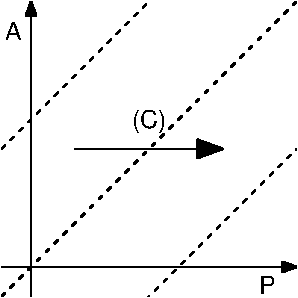
\includegraphics[height = 2cm]{../fig/APc.pdf} &
  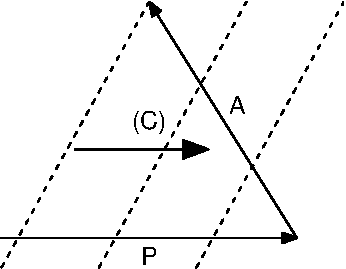
\includegraphics[height = 2cm]{../fig/APc_iso.pdf}  \\
  %%%% ACp
  $$\begin{aligned}
    &AC(P) \\
    &P = C + A
  \end{aligned}$$ &
  The $AC(P)$ temporal plane is equivalent to the Lexis diagram only that birth cohort is given and period is embedded instead of the other way round. &
  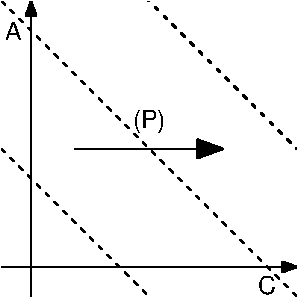
\includegraphics[height = 2cm]{../fig/ACp.pdf} &
  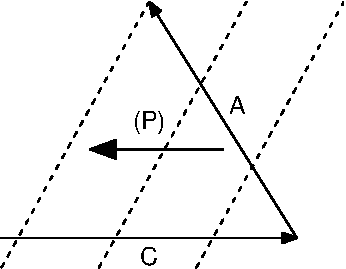
\includegraphics[height = 2cm]{../fig/ACp_iso.pdf}  \\
  %%%% CPa
  $$\begin{aligned}
    &CP(A) \\
    &A = P - C
  \end{aligned}$$ &
  The $CP(A)$ temporal plane is equivalent to the Lexis diagram only that birth cohort is given and age is embedded instead of the other way round. &
  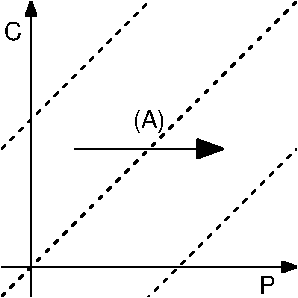
\includegraphics[height = 2cm]{../fig/CPa.pdf} &
  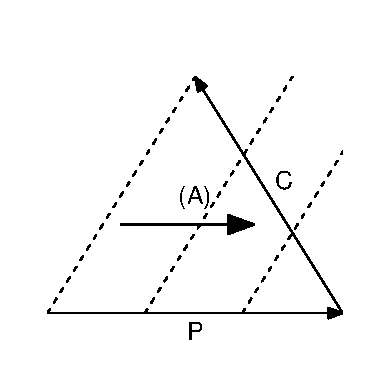
\includegraphics[height = 2cm]{../fig/CPa_iso.pdf}  \\
  \midrule
  %%%%%%%%%%%%%%%%%%%%%%%%%%%%%%%%%%%%%%%%%%%%%%%%%%%%%%%%%%%%%%%%%%%%%%%%%%%%%
  \multicolumn{4}{c}{\textsc{Variants of TPD}} \\
  \midrule
  %%%% TPd
  $$\begin{aligned}
    &TP(D) \\
    &D = P + T
  \end{aligned}$$ &
  Helen had 30 years of life left ($T$) in 1971 ($P$) and therefore belonged to the 2001 death cohort ($D$) &
  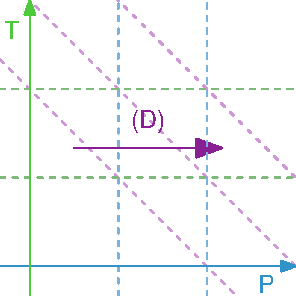
\includegraphics[height = 2cm]{../fig/TPd.pdf} &
  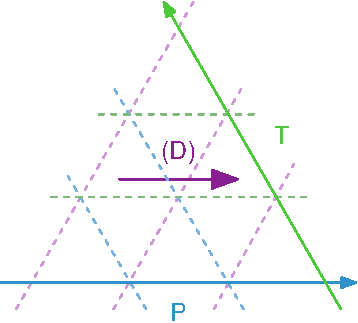
\includegraphics[height = 2cm]{../fig/TPd_iso.pdf}  \\
  %%%% PDt
  $$\begin{aligned}
    &PD(T) \\
    &T = D - P
  \end{aligned}$$ &
  Mindel died in 1973 ($D$). In 1953 ($P$) she had 20 years left to live ($T$). &
  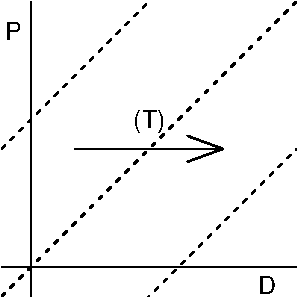
\includegraphics[height = 2cm]{../fig/PDt.pdf} &
  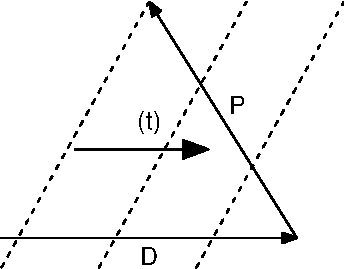
\includegraphics[height = 2cm]{../fig/PDt_iso.pdf}  \\
  %%%% TDp
  $$\begin{aligned}
    &TD(P) \\
    &P = D - T
  \end{aligned}$$ &
  Irene died in 1974 ($D$). When she had 30 remaining years of life ($T$) the year must have been 1944 ($P$). &
  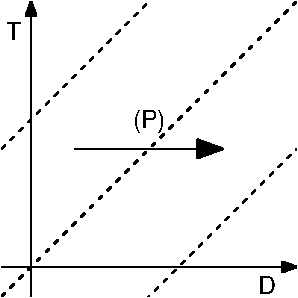
\includegraphics[height = 2cm]{../fig/TDp.pdf} &
  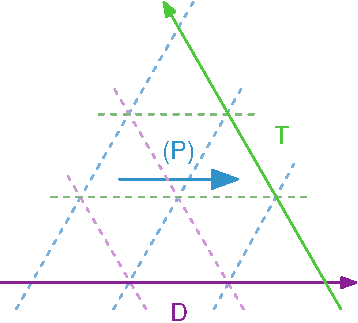
\includegraphics[height = 2cm]{../fig/TDp_iso.pdf}  \\
  \midrule
  %%%%%%%%%%%%%%%%%%%%%%%%%%%%%%%%%%%%%%%%%%%%%%%%%%%%%%%%%%%%%%%%%%%%%%%%%%%%%
  \multicolumn{4}{c}{\textsc{Variants of TAL}} \\
  \midrule
  %%%% TAl
  $$\begin{aligned}
    &TA(L) \\
    &L = T + A
  \end{aligned}$$ &
  The time already lived and the time still left sum up to the total lifespan. &
  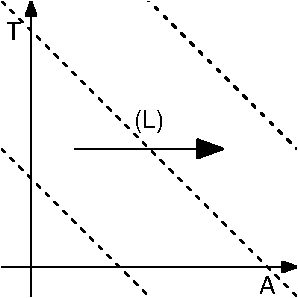
\includegraphics[height = 2cm]{../fig/TAl.pdf} &
  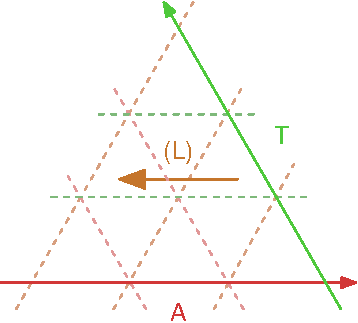
\includegraphics[height = 2cm]{../fig/TAl_iso.pdf}  \\
  %%%% TLa
  $$\begin{aligned}
    &TL(A) \\
    &A = L - T
  \end{aligned}$$ &
  Helen lived to the age of 86 ($L$). When she had 20 years left ($T$) she must have been 66 ($A$). &
  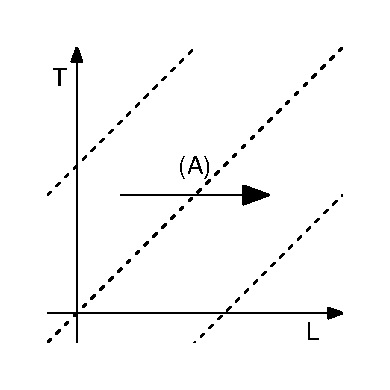
\includegraphics[height = 2cm]{../fig/TLa.pdf} &
  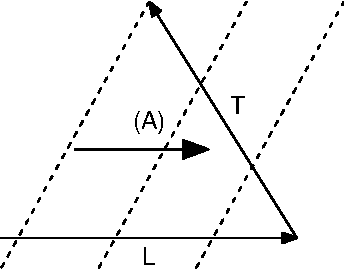
\includegraphics[height = 2cm]{../fig/TLa_iso.pdf}  \\
  %%%% ALt
  $$\begin{aligned}
    &AL(T) \\
    &T = A - L
  \end{aligned}$$ &
  Tim is 34 years old ($A$) and will live to the age of 96 ($L$), leaving him 62 years ($T$) to settle affairs. &
  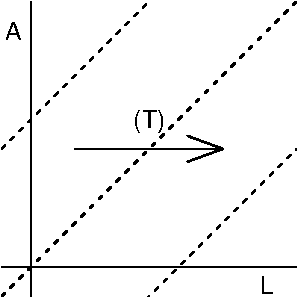
\includegraphics[height = 2cm]{../fig/ALt.pdf} &
  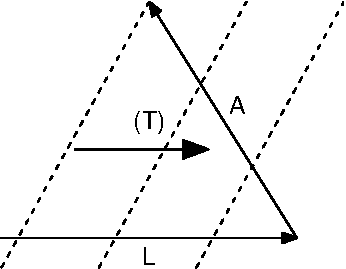
\includegraphics[height = 2cm]{../fig/ALt_iso.pdf}  \\
  \midrule
  %%%%%%%%%%%%%%%%%%%%%%%%%%%%%%%%%%%%%%%%%%%%%%%%%%%%%%%%%%%%%%%%%%%%%%%%%%%%%
  \multicolumn{4}{c}{\textsc{Variants of LCD}} \\
  \midrule
  %%%% LCd
  $$\begin{aligned}
    &LC(D) \\
    &D = C + L
  \end{aligned}$$ &
  Àngels was born in 1940 ($C$) and she lived to be 64 ($L$), implying an
  untimely death in 2004 ($D$) &
  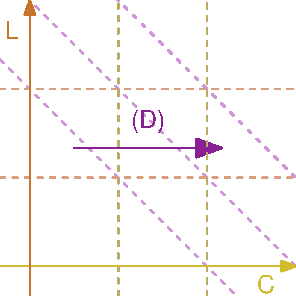
\includegraphics[height = 2cm]{../fig/LCd.pdf} &
  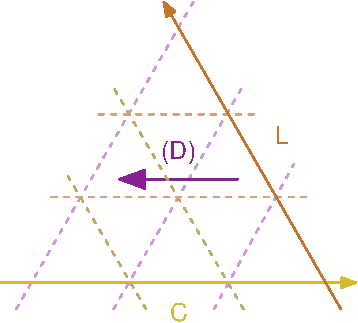
\includegraphics[height = 2cm]{../fig/LCd_iso.pdf}  \\
  %%%% CDl
  $$\begin{aligned}
    &CD(L) \\
    &L = D - C
  \end{aligned}$$ &
  Pascal was born in 1893 ($C$) and died in 1964 ($D$), implying a lifespan of 71 ($L$), or so. &
  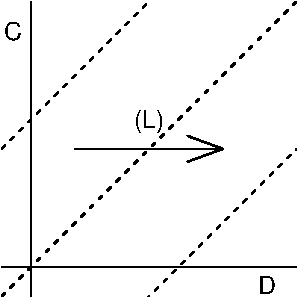
\includegraphics[height = 2cm]{../fig/CDl.pdf} &
  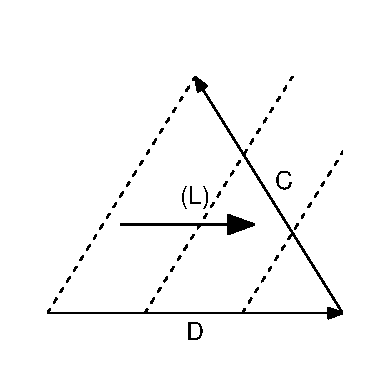
\includegraphics[height = 2cm]{../fig/CDl_iso.pdf}  \\
  %%%% LDc
  $$\begin{aligned}
    &LD(C) \\
    &C = D - L
  \end{aligned}$$ &
  Margaret died in Dec., 1995 ($D$) with a completed lifespan of 96 ($L$), putting her birth year in 1900 ($C$). &
  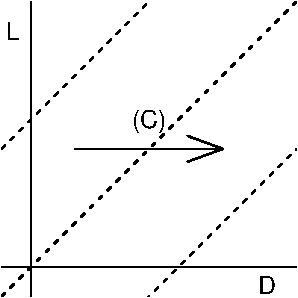
\includegraphics[height = 2cm]{../fig/LDc.pdf} &
  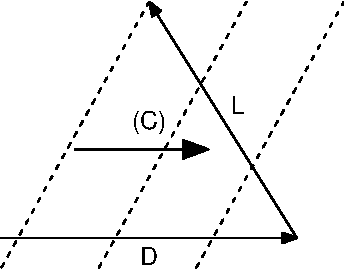
\includegraphics[height = 2cm]{../fig/LDc_iso.pdf}  \\
  \midrule
  %%%%%%%%%%%%%%%%%%%%%%%%%%%%%%%%%%%%%%%%%%%%%%%%%%%%%%%%%%%%%%%%%%%%%%%%%%%%%
  \multicolumn{4}{c}{\textsc{2-D Combinations of Lexis Scales and Thanatological Scales}} \\
  \midrule
  %%%% LP
  $LP(-)$ &
  The $LP$ plane is \emph{non-informative}. No additional dimensions can be derived knowing just lifespan and period. &
  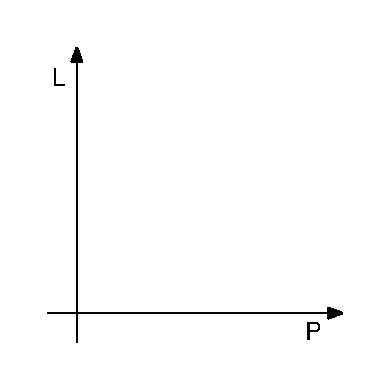
\includegraphics[height = 2cm]{../fig/LP.pdf} &
  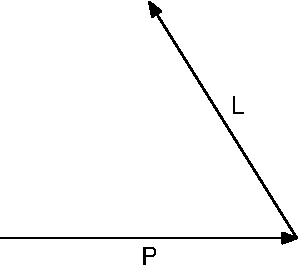
\includegraphics[height = 2cm]{../fig/LP_iso.pdf}  \\
  %%%% CT
  $CT(-)$ &
  The $CT$ plane is \emph{non-informative}. No additional dimensions can be derived knowing just cohort and thanatological age. &
  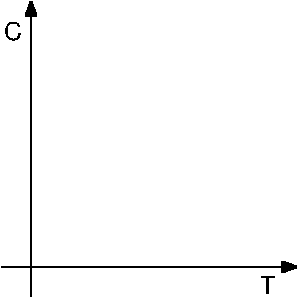
\includegraphics[height = 2cm]{../fig/CT.pdf} &
  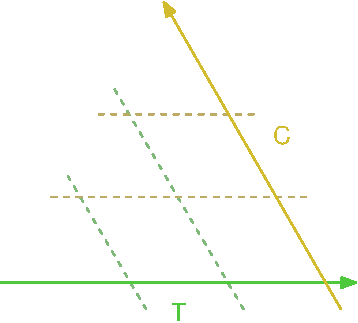
\includegraphics[height = 2cm]{../fig/CT_iso.pdf}  \\
  %%%% AD
  $AD(-)$ &
  The $AD$ plane is \emph{non-informative}. No additional dimensions can be derived knowing just death cohort and age. &
  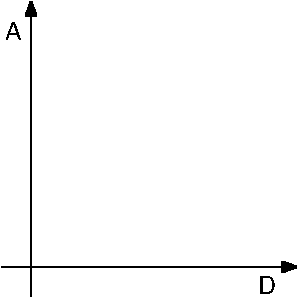
\includegraphics[height = 2cm]{../fig/AD.pdf} &
  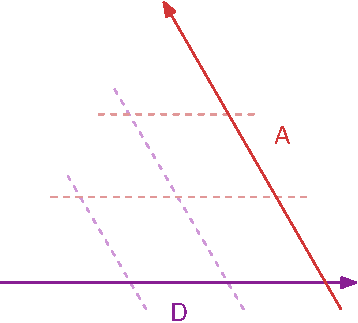
\includegraphics[height = 2cm]{../fig/AD_iso.pdf}  \\
  \bottomrule
  \end{longtable}
\end{center}

\clearpage

\end{document}